\chapter{Modellierung}
\section{UND-Operation}
\subsection{Erster Ansatz}
\begin{figure}[ht]
    \centering
    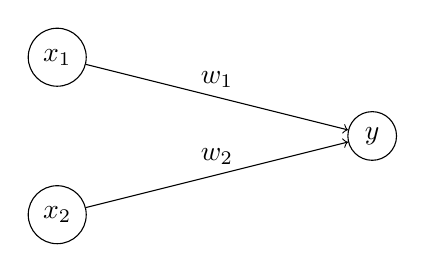
\begin{tikzpicture}
        \node[shape=circle,draw=black] (x1) at (0,0) {$x_1$};
        \node[shape=circle,draw=black] (x2) at (0,-2) {$x_2$};
        \node[shape=circle,draw=black] (y) at (4,-1) {$y$};

        \path [->] (x1) edge node[above] {$w_1$} (y);
        \path [->] (x2) edge node[above] {$w_2$} (y);
    \end{tikzpicture}
    \caption{Erster Ansatz}
    \label{fig:net0}
\end{figure}

\begin{flushleft}   
Der erste Ansatz eines neuronalen Netzes ist in Abbildung \ref{fig:net0} dargestellt.
Das Ergebnis ($y$) setzt sich wie folgt zusammen:
\begin{align}
    y&=x_1w_1+x_2w_2 \\
    y&=\begin{pmatrix} x_1 \\ x_2 \end{pmatrix}\cdot\begin{pmatrix} w_1 \\ w_2 \end{pmatrix}
\end{align}

Um dieses Netz auf die UND-Operation zu trainieren, können alle Werte aus der Tabelle aus Abbildung \ref{fig:or} eingesetzt werden.
\begin{align}
    \text{I:}&\quad 0=\begin{pmatrix}
        0 \\
        0
    \end{pmatrix}\cdot
    \begin{pmatrix}
        w_1 \\
        w_2
    \end{pmatrix}=0 \\
    \text{II:}&\quad 0=\begin{pmatrix}
        0 \\
        1
    \end{pmatrix}\cdot
    \begin{pmatrix}
        w_1 \\
        w_2
    \end{pmatrix}=w_2 \\
    \text{III:}&\quad 0=\begin{pmatrix}
        1 \\
        0
    \end{pmatrix}\cdot
    \begin{pmatrix}
        w_1 \\
        w_2
    \end{pmatrix}=w_1 \\
    \text{IIII:}&\quad 1=\begin{pmatrix}
        1 \\
        1
    \end{pmatrix}\cdot
    \begin{pmatrix}
        w_1 \\
        w_2
    \end{pmatrix}=w_1+w_2
\end{align}

Schnell wird klar, dass das Gleichungssystem keine Lösung hat.
\begin{align}
    0&=w_1 \\
    0&=w_2 \\
    1&=w_1+w_2
\end{align}
\end{flushleft}

\subsection{Der Bias}
\begin{flushleft}
Der nächste logische Schritt ist einen sogenannten \say{bias} zu nutzen,
um mehr Parameter im Gleichungssystem zu haben, die verändert werden dürfen.
\end{flushleft}

\begin{figure}[ht]
    \centering
    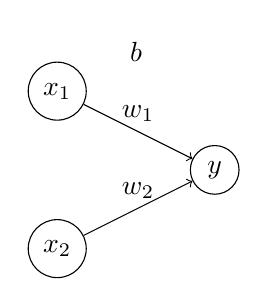
\begin{tikzpicture}
        \node[shape=circle,draw=black] (x1) at (0,0) {$x_1$};
        \node[shape=circle,draw=black] (x2) at (0,-2) {$x_2$};
        \node[shape=circle,draw=black] (y) at (2,-1) {$y$};
        \node[shape=circle,draw=none] (b) at (1,0.5) {$b$};

        \path [->] (x1) edge node[above] {$w_1$} (y);
        \path [->] (x2) edge node[above] {$w_2$} (y);
    \end{tikzpicture}
    \caption{Modell mit Bias}
    \label{fig:net1}
\end{figure}

\begin{flushleft}
Für die Abbildung \ref{fig:net1} gilt folgendes:
\begin{align}
    y&=x_1w_1+x_2w_2+b \\
    y&=\begin{pmatrix}
        x_1 \\
        x_2
    \end{pmatrix}\cdot
    \begin{pmatrix}
        w_1 \\
        w_2
    \end{pmatrix}+b
\end{align}

Es ergeben sich also die folgenden Gleichungen:
\begin{align}
    \text{I:}&\quad 0=\begin{pmatrix}
        0 \\
        0
    \end{pmatrix}\cdot
    \begin{pmatrix}
        w_1 \\
        w_2
    \end{pmatrix}+b=b \\
    \text{II:}&\quad 0=\begin{pmatrix}
        0 \\
        1
    \end{pmatrix}\cdot
    \begin{pmatrix}
        w_1 \\
        w_2
    \end{pmatrix}+b=w_2+b \\
    \text{III:}&\quad 0=\begin{pmatrix}
        1 \\
        0
    \end{pmatrix}\cdot
    \begin{pmatrix}
        w_1 \\
        w_2
    \end{pmatrix}+b=w_1+b \\
    \text{IIII:}&\quad 1=\begin{pmatrix}
        1 \\
        1
    \end{pmatrix}\cdot
    \begin{pmatrix}
        w_1 \\
        w_2
    \end{pmatrix}+b=w_1+w_2+b
\end{align}

Nun fällt auf, dass diese Gleichungen exakt den vorherigen Gleichungen entsprechen, da die erste Gleichung wie folgt lautet:
\begin{align}
    \text{I:}\quad b=0
\end{align}   
\end{flushleft}

\subsection{Sigmoidfunktion}
\begin{flushleft}   
Das nächste Problem der Modellierung ist, dass für $y$ bisher nur exakte Werte genutzt wurden.
Jedoch wäre es eigentlich egal, ob beispielsweise bei der ersten Gleichung für $y$ der Wert $0.00001$, oder eben der exakte Wert $0$ herauskommt.
Relevant ist, dass $y$ der $0$ relativ nahe kommt.

Dies kann durch den Einsatz der Sigmoidfunktion erreicht werden.

$sig(t)$, oder alternativ $\sigma(t)$, ist wie folgt definiert:
\begin{align}
    \sigma(t)=\frac{1}{1+e^{-t}}
\end{align}
\end{flushleft}

\begin{figure}[ht]
    \centering
    \begin{tikzpicture}
    \begin{axis}[
        axis lines=left,
        xlabel=$x$,
        xmin=-8,
        xmax=8,
        ylabel=$\sigma(x)$,
        ymin=0,
        ymax=1
        ]
        \addplot[domain=-8:8,color=blue] {1/(1+exp(-x))};
    \end{axis}
    \end{tikzpicture}
    \caption{Plot der Sigmoidfunktion für $x\in\left[-8,8\right]$}
    \label{fig:sigplot}
\end{figure}

\begin{flushleft}   
Die Sigmoidfunktion eignet sich perfekt um Werte auf das Interval $\left]0,1\right[$ zu bringen.

Es gilt nämlich:
\begin{align}
    \lim_{x\to-\infty} \sigma(x) = 0 \\
    \lim_{x\to\infty} \sigma(x) = 1
\end{align}

Die Sigmoidfunktion kann also helfen eine Lösung für das Gleichungssystem zu finden.
\end{flushleft}

\begin{figure}[ht]
    \centering
    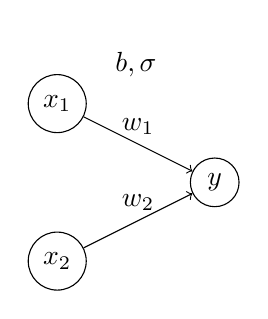
\begin{tikzpicture}
        \node[shape=circle,draw=black] (x1) at (0,0) {$x_1$};
        \node[shape=circle,draw=black] (x2) at (0,-2) {$x_2$};
        \node[shape=circle,draw=black] (y) at (2,-1) {$y$};
        \node[shape=circle,draw=none] (b) at (1,0.5) {$b,\sigma$};

        \path [->] (x1) edge node[above] {$w_1$} (y);
        \path [->] (x2) edge node[above] {$w_2$} (y);
    \end{tikzpicture}
    \caption{Modell mit Bias und Sigmoidfunktion}
    \label{fig:net2}
\end{figure}

\begin{flushleft}
Das in Abbildung \ref{fig:net2} gezeigte Modell nutzt die Sigmoidfunktion um $y$ zu berechnen:
\begin{align}
    y&=\sigma(x_1w_1+x_2w_2+b) \\
    y&=\sigma\left(\begin{pmatrix}
        x_1 \\
        x_2
    \end{pmatrix}\cdot
    \begin{pmatrix}
        w_1 \\
        w_2
    \end{pmatrix}+b\right) \\
    \text{I:}&\quad 0=\sigma\left(\begin{pmatrix}
        0 \\
        0
    \end{pmatrix}\cdot
    \begin{pmatrix}
        w_1 \\
        w_2
    \end{pmatrix}+b\right)=\sigma(b) \\
    \text{II:}&\quad 0=\sigma\left(\begin{pmatrix}
        0 \\
        1
    \end{pmatrix}\cdot
    \begin{pmatrix}
        w_1 \\
        w_2
    \end{pmatrix}+b\right)=\sigma(w_2+b) \\
    \text{III:}&\quad 0=\sigma\left(\begin{pmatrix}
        1 \\
        0
    \end{pmatrix}\cdot
    \begin{pmatrix}
        w_1 \\
        w_2
    \end{pmatrix}+b\right)=\sigma(w_1+b) \\
    \text{IIII:}&\quad 1=\sigma\left(\begin{pmatrix}
        1 \\
        1
    \end{pmatrix}\cdot
    \begin{pmatrix}
        w_1 \\
        w_2
    \end{pmatrix}+b\right)=\sigma(w_1+w_2+b)
\end{align}

Da $\sigma(b)=0$ nur für $b=-\infty$ gilt und ein echter Wert für $b$ gefordert wird, müssen die Gleichungen leicht verändert werden.
\begin{align}
    \text{I:}&\quad 0\approx\sigma(b) \\
    \text{II:}&\quad 0\approx\sigma(w_2+b) \\
    \text{III:}&\quad 0\approx\sigma(w_1+b) \\
    \text{IIII:}&\quad 1\approx\sigma(w_1+w_2+b)
\end{align}

Anhand von der Abbildung \ref{fig:sigplot} lässt sich erkennen, dass:
\begin{align}
    \sigma(x)\approx0\quad \forall x< -8
\end{align}

Nimmt man sich also eine beliebige Zahl, die kleiner als $-8$ ist, beispielsweise $-10$, muss gelten:
\begin{align}
    b\leq -10,&\quad\text{da}\quad\sigma(x)\approx 0\quad\forall x\leq -10 \\
    w_2+b\leq -10,&\quad\text{da}\quad\sigma(x)\approx 0\quad\forall x\leq -10 \\
    w_1+b\leq -10,&\quad\text{da}\quad\sigma(x)\approx 0\quad\forall x\leq -10 \\
    w_1+w_2+b\geq 10,&\quad\text{da}\quad\sigma(x)\approx 1\quad\forall x\geq 10
\end{align}

Dieses System von Ungleichungen hat unendlich viele Lösungen:
\begin{align}
    w_2=20,\quad b\leq -30,\quad w_1=-10-b
\end{align}

Hier ist jedoch nur eine relevant:
\begin{align}
    w_2=20,\quad b=-30,\quad w_1=20
\end{align}

Für diese Lösung gilt also:
\begin{align}
    \sigma(-30)&=\frac{1}{1+e^{30}}\approx 0 \\
    \sigma(20-30)&=\sigma(-10)=\frac{1}{1+e^{10}}\approx 0 \\
    \sigma(20-30)&=\sigma(-10)=\frac{1}{1+e^{10}}\approx 0 \\
    \sigma(20+20-30)&=\sigma(10)=\frac{1}{1+e^{\frac{1}{10}}}\approx 1
\end{align}

Somit ist eine Lösung des Modells:
\begin{align}
    y&=\sigma\left(\begin{pmatrix}
        x_1 \\
        x_2
    \end{pmatrix}\cdot
    \begin{pmatrix}
        20 \\
        20
    \end{pmatrix}-30\right)
\end{align}
\end{flushleft}

\section{ODER-Operation}
\begin{flushleft}
Grundsätzlich ist das Modell der ODER-Operation, gleich dem in Abbildung \ref{fig:net2} gezeigten Modell.

Somit gilt also auch:
\begin{align}
    y&=\sigma\left(\begin{pmatrix}
        x_1 \\
        x_2
    \end{pmatrix}\cdot
    \begin{pmatrix}
        w_1 \\
        w_2
    \end{pmatrix}+b\right)
\end{align}

Es ergeben sich die folgenden Gleichungen:
\begin{align}
    \text{I:}&\quad 0\approx\sigma(b) \\
    \text{II:}&\quad 1\approx\sigma(w_2+b) \\
    \text{III:}&\quad 1\approx\sigma(w_1+b) \\
    \text{IIII:}&\quad 1\approx\sigma(w_1+w_2+b)
\end{align}

Wenn man der vorherigen Annahme, dass $\sigma(-10)\approx 0,\sigma(10)\approx 1$ gilt, folgt sind hier die passenden Ungleichungen:
\begin{align}
    b\leq -10,&\quad\text{da}\quad\sigma(x)\approx 0\quad\forall x\leq -10 \\
    w_2+b\geq 10,&\quad\text{da}\quad\sigma(x)\approx 1\quad\forall x\geq 10 \\
    w_1+b\geq 10,&\quad\text{da}\quad\sigma(x)\approx 1\quad\forall x\geq 10 \\
    w_1+w_2+b\geq10,&\quad\text{da}\quad\sigma(x)\approx 1\quad\forall x\geq 10
\end{align}

Wie auch beim Modell der UND-Operation, gibt es hier unendlich viele Lösungen:
\begin{align}
    b=-10,\quad w_2=20,\quad w_1\geq 20
\end{align}

Also gelten die Gleichungen für beispielsweise:
\begin{align}
    b=-10,&\quad w_2=20,\quad w_1=20 \\
    \text{I:}&\quad 0\approx\sigma(-10) \\
    \text{II:}&\quad 1\approx\sigma(10) \\
    \text{III:}&\quad 1\approx\sigma(10) \\
    \text{IIII:}&\quad 1\approx\sigma(30)
\end{align}

Die ODER-Operation kann also durch die folgende Funktion $y$ in Abhängigkeit von $x_1$ und $x_2$ modelliert werden:
\begin{align}
    y&=\sigma\left(\begin{pmatrix}
        x_1 \\
        x_2
    \end{pmatrix}\cdot
    \begin{pmatrix}
        20 \\
        20
    \end{pmatrix}-10\right)
\end{align}
\end{flushleft}
